%%% -*- TeX-master: "../main" -*-
\chapter{From Time Series to Label Sequences}
\label{cha:methods}

\begin{figure}[h]
  % Center this figure specifically because it is wider than \textwidth
  \makebox[\textwidth][c]{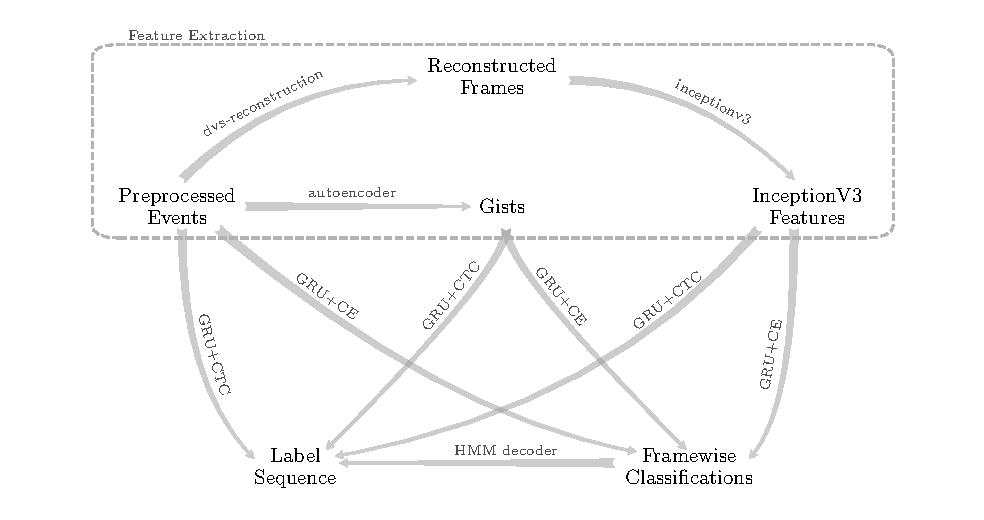
\includegraphics{figures/methods/overview}}
  \caption{Overview of the methods and intermediate representations used in this
    thesis}
  \label{fig:method-overview}
\end{figure}

There are three types of sequence labeling tasks defined by Graves. The first is
sequence classification where the data is a set of sequences each of which
belongs to a single class. This problem can be generalized to segment
classification. Here a data point is subdivided into one or more segments with
known start and end points and each of them needs to be classified. Splitting
the inputs along the segment boundaries and interpreting the problem as a
sequence classification task is not equivalent because the segment classifier
may and often will use surrounding context to disambiguate ambiguous segments.
The most general task is called temporal classification in which neither the
number of classes per sequence nor any segment boundaries are known. The only
assumption is that an input has at most as many labels as the length of the
input sequence. Such a classifier has to compute just the label sequence, though
some of them can optionally also return a segmentation.

The problem of gesture recognition from address-event data falls into the last
category. A recording may contain any number of gestures at arbitrary points in
time and each gesture takes up a varying number of events depending on distance
between hand and DVS, speed of execution and lighting conditions. Figure
\ref{fig:method-overview} depicts all the ways that we tried to solve this
temporal classification task. All of them include recurrent neural networks
(RNNs) because they are the state of the art in sequence learning. There are two
popular ways to compute a label sequence from an input. The older one combines
an RNN and a hidden Markov model (HMM). The RNN provides localized
classifications of each sequence element and the HMM segments the input on the
basis of the RNN output and deduces the most likely label sequence. These are
all paths in Figure \ref{fig:method-overview} that leave the feature extraction
phase and take \emph{framewise classifications} as an intermediate step to
\emph{label sequence}. \citeauthor{ctc} devised a method called connectionist
temporal classification (CTC) that combines both steps, RNN classification and
HMM decoding, by means of a new loss function for neural network training. This
enables a neural network in theory to solve any temporal classification task
end-to-end. This approach is represented in Figure \ref{fig:method-overview} by
all paths labeled \texttt{GRU+CTC} that lead to \emph{label sequence} directly.

Neural networks that are capable of sequence-to-sequence transformations rely on
circular connections in their computational graph and are called recurrent
neural networks. They process an input sequence element by element and the
recurrent connections allow them to carry information, and thus context, from
step to step. The particular variant of RNN we use is called a gated recurrent
unit, GRU for short, which allows the networks to learn much longer temporal
relationships than a naive RNN could. We introduce RNNs, GRUs and their
predecessor, the long short-term memory layer, in Section \ref{sec:rnns}.

In the beginning, we applied both methods to the 25-gesture dataset, however CTC
training did not produce any result at all and framewise classification levelled
off at about 40\% accuracy, which we deemed to low for successful decoding. The
type of data that we are handling consists of very long sequences with only
minimal information content per sequence element and a high noise ratio. The
recordings average 30,000 events per second and single gestures often span over
100,000 events. Even though we employ gated recurrent units that can learn
relationships over hundreds of timesteps, we assumed that the network might be
just overwhelmed by the data. Moreover, we conjectured that the continuous time
and consequential variance in event density over time made the task more
difficult. We introduced two feature extraction methods with the specific goal
of overcoming these problems. Both compress sequences of varying length into
fixed-length vectors. That lets us transform the continuous-time sequences into
discrete-time ones by grouping the events into time windows of fixed length but
varying numbers of events and compress them into fixed-length vectors. The
transformed sequences should improve learning because the number of data points
per second is cut down and the data points are enriched with the information of
all events then went into them. On the original data, the network had to rely
almost purely on the context, because a single event is uninformative.
Afterwards, each data point should be quite meaningful on its own.

% TODO: Train CNN classifier on gists to check how much context is actually
% necessary

The first method reconstructs grayscale images from the event data (Section
\ref{sec:frame-reconstruction}) and then uses a pre-trained image classification
network to extract visual features (Section \ref{sec:inceptionv3}). The second
idea, explained in Section \ref{sec:autoencoder}, uses a specific type of
network, an autoencoder, to learn an efficient compression directly. We call the
representations learned by the autoencoder \emph{gists} because they encode the
gist of the input.

Section \ref{sec:framewise} explains framewise classification and how a network
is trained for that. These local classifications are decoded with an HMM and
some custom post-processing which is described in Section \ref{sec:hmm}. Lastly,
we introduce connectionist temporal classification in Section \ref{sec:ctc} and
explain how it combines the steps of classification and decoding into one.

\section{Recurrent Neural Networks}
\label{sec:rnns}

The classical neural network is a parametric function approximator that takes an
input vector of fixed length and produces an output vector of fixed length.
Recurrent neural networks generalize either input, output or both to sequences.
Let $x^{(n)}$ be a sequence of input vectors and define a simple network with
one hidden layer. So it has a weight matrices $W$, $V$, a bias $b$ and in this
example we will use a $\tanh$ non-linearity. The naive way to produce an output
sequence $y^{(n)}$ would be to apply the network elementwise by
\begin{align*}
  h^{(t)} & = \tanh\left( Wx^{(t)} + b \right)\\
  y^{(t)} & = Vh^{(t)}
\end{align*}
where $h^{(t)}$ are the activations in the hidden layer for the $t$-th sequence
element. However, this network does not have access to any historical context
and so it will have a difficult time to, for example, recognize gestures which
are inherently temporal. One solution is to introduce recurrent connections
between layers in the form of an additional dependency of $h^{(t)}$ on $h^{(t -
  1)}$. In precise terms this means that we add another weight matrix $U$ to the
network and redefine it as
\begin{align*}
  h^{(t)} & = \tanh\left( Wx^{(t)} + Uh^{(t - 1)} + b \right)\\
  y^{(t)} & = Vh^{(t)}
\end{align*}
where $h^{(0)}$ is initialized arbitrarily, though with the zero vector most of
the time. This network now has memory, so to speak, in the form of $h^{(t)}$
that allows it to take the history of the sequence into account.

Though fine in theory, in practice this type of RNN suffers from the vanishing
gradient problem. When such a network is trained with some form of gradient
descent, the gradient decays exponentially quickly as it propagates back through
time. This makes it hard for such a network to solve tasks that require more
than about 10 steps of temporal contrast. \citeauthor{lstm} solved this with the
introduction of long short-therm memory (LSTM) layers that they designed to
allow constant error flow \cite{lstm}. Instead of carrying over the state of the
hidden layer directly, the LSTM architecture replaces the hidden layer with a
subnetwork that explicitly controls which memories should be forgotten and which
should be overwritten. This keeps the gradient magnitude large and provides
sufficient signal for learning over several hundred timesteps. An LSTM layer
consists of two persistent states, the cell state $c^{(t)}$ and the hidden state
$h^{(t)}$, and three gates, the input, output and forget gates $i^{(t)}$,
$o^{(t)}$ and $f^{(t)}$, respectively, which control the flow of information.
They are connected as follows where $\sigma$ is the logistic sigmoid function
and $\circ$ denotes an element-wise product.
% TODO: Explain the logistic sigmoid?
\begin{align*}
  f^{(t)} & = \sigma\left( W_{f}x^{(t)} + U_{f}h^{(t - 1)} + b_{f} \right)\\
  i^{(t)} & = \sigma\left( W_{i}x^{(t)} + U_{i}h^{(t - 1)} + b_{i} \right)\\
  o^{(t)} & = \sigma\left( W_{o}x^{(t)} + U_{o}h^{(t - 1)} + b_{o} \right)\\
  c^{(t)} & = f^{(t)} \circ c^{(t - 1)} + i^{(t)} \circ \tanh\left( W_{c}x^{(t)} + U_{c}h^{(t - 1)} + b_{c} \right)\\
  h^{(t)} & = o^{(t)} \circ \tanh\left( c^{(t)} \right)
\end{align*}
The forget and input gates control the updates to the cell state while the
output gate controls which parts of the cell state are written out into the
hidden state and thus into the output of the layer. A later version called
Peephole LSTM uses the cell state directly instead of the previous hidden state
to compute the input, output and forget gates.

% TODO: tikz pictures of RNN, LSTM and GRU computational graphs

In \citeyear{gru} \citeauthor{gru} published a simplification of LSTM called a
gated recurrent unit (GRU) \cite{gru}. They merge the cell state into the hidden
state $h^{(t)}$, combine the input and forget gates into a single update gate
$z^{(t)}$ and replace the output gate with a reset gate $r^{(t)}$ that has no
equivalent in LSTM. A GRU layer is then defined by
% TODO: Mention z and (1 - z)
\begin{align*}
  r^{(t)} & = \sigma\left( W_{r}x^{(t)} + U_{r}h^{(t - 1)} \right)\\
  z^{(t)} & = \sigma\left( W_{z}x^{(t)} + U_{z}h^{(t - 1)} \right)\\
  h^{(t)} & = z^{(t)} \circ h^{(t - 1)} + \left( 1 - z^{(t)} \right) \circ \tilde{h}^{(t)}\\
  \tilde{h}^{(t)} & = \tanh\left( Wx^{(t)} + U\left( r^{(t)} \circ h^{(t - 1)} \right) \right).
\end{align*}
where $\tilde{h}^{(t)}$ is an intermediate variable. This architecture has fewer
parameters and operations then LSTM which makes it easier to implement and
compute which reduces training time. \citeauthor{gruvslstm} have found that GRU
performance is comparable to LSTM \cite{gruvslstm}. For these reasons, we have
decided to rely on GRUs in this thesis.

\section{Frame Reconstruction}
\label{sec:frame-reconstruction}

The DVS only reacts to changes in light intensity. This removes all the
redundant information about stationary objects that makes up the bulk of the
data in videos consisting of consecutive frames. Furthermore, the remaining
information about the illumination gradient at a point is coarsely discretized
and carries just a single bit of information, the sign of the change.
Nonetheless, two groups have shown that it is still possible to reconstruct
grayscale images from the data \cite{bardow2016,reinbacher2016}.
\citeauthor{reinbacher2016} interpret the events as points on an event manifold
which they reconstruct by minizing an energy including a smoothness regularizer
over it with variational methods. The solution can then be interpreted as an
intensity image.

They have published an open-source implementation of their algorithm which we
used to reconstruct images from the dataset. We created one image every
\SI{2.5}{\milli\second} resulting in 400 frames per second. Figure
\ref{fig:reconstructed} showcases three frames depicting a \texttt{swipe-down}
gesture. For one thing, the subject's hand has been resolved reasonable well and
it has been reconstructed as one smooth surfaces with shadows creating an
illusion of depth and even individual digits are visible. At the same time
though, artifacts are accumulating in the background regions of the image and
over time the images become darker. The reason for this is most likely that we
mounted the camera on a stand. As a result it was static relative to the
background which therefore produced no events.

\begin{figure}[h]
  \centering
  \begin{subfigure}{\textwidth}
    \hspace*{\fill}
    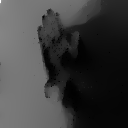
\includegraphics[width=0.3\textwidth]{figures/methods/reconstructed-1}
    \hspace*{\fill}
    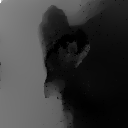
\includegraphics[width=0.3\textwidth]{figures/methods/reconstructed-2}
    \hspace*{\fill}
    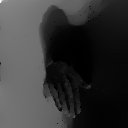
\includegraphics[width=0.3\textwidth]{figures/methods/reconstructed-3}
    \hspace*{\fill}
  \end{subfigure}
  \caption{Reconstructed frames showing a \texttt{swipe-down} gesture}
  \label{fig:reconstructed}
\end{figure}

\section{Feature Extraction with an InceptionV3 Network}
\label{sec:inceptionv3}

It is an emergent property of neural networks trained on image tasks that they
develop increasingly abstract features in higher levels of the network. So the
bottom layers of a network will learn to recognize simple shapes like edges in
various orientations or corners. On top of these, the network learns to
recognize more complex shapes like circles or rectangles. This continues through
the network and in the highest layers you find neurons that recognize faces or
cars. An insight from transfer learning says that these learned features can be
reused across a variety of tasks because only a handful of layers at the top
will be completely task specific. So by reusing a pre-trained network and
replacing the top layers you can reach high performance on a new task in a
fraction of the time it would take to train the whole network from scratch. In
our case, reusing a network pre-trained on a large dataset has the additional
advantage that we can indirectly make use of a lot more training data than what
our dataset provides.

\begin{figure}[h]
  \centering
  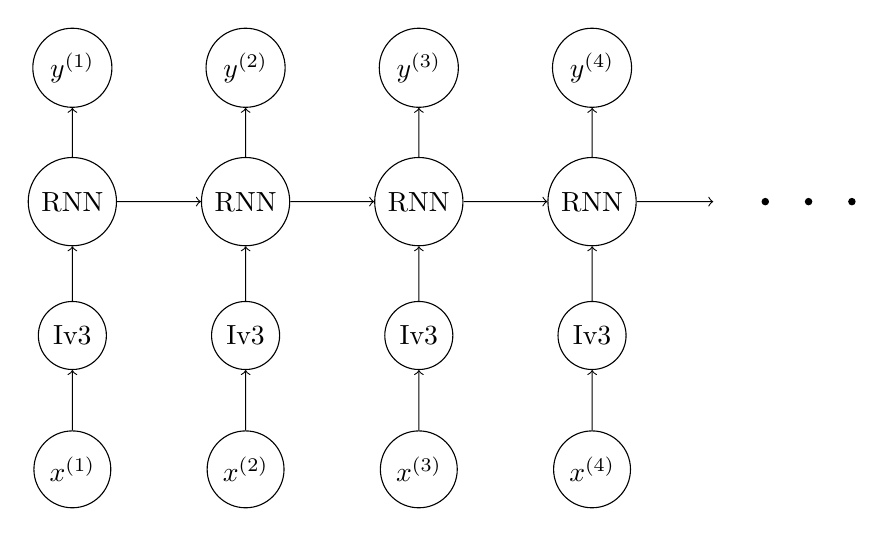
\begin{tikzpicture}[xscale=2.2,yscale=1.7]
    \foreach \t in {1, 2, 3, 4} {
      \node[draw,circle](x\t) at (\t, 0) {$x^{(\t)}$};
      \node[draw,circle](i\t) at (\t, 1) {Iv3};
      \node[draw,circle](r\t) at (\t, 2) {RNN};
      \node[draw,circle](y\t) at (\t, 3) {$y^{(\t)}$};

      \draw[->] (x\t) -- (i\t);
      \draw[->] (i\t) -- (r\t);
      \draw[->] (r\t) -- (y\t);
    }

    \foreach \t [evaluate=\t as \tnext using int(\t + 1)] in {1, 2, 3} {
      \draw[->] (r\t) -- (r\tnext);
    }

    \draw[->] (r4) -- (4.7,2);
    \foreach \p [evaluate=\p as \x using (5 + 1/4 * \p)] in {0, 1, 2} {
      \fill (\x, 2) node[draw,circle,fill,inner sep=0,minimum size=0.08cm]{};
    }
  \end{tikzpicture}
  \caption{Computational graph of an RNN on top of an InceptionV3 network}
  \label{fig:iv3-rnn}
\end{figure}

The end goal is to compress sequences of events into more expressive data
points. The idea for that is that we reconstruct grayscale images from the event
data and then feed these to a pre-trained network that is able to extract
abstract and meaningful features about the subjects hand position from them. In
particular, we chose an InceptionV3 network \cite{inceptionv3} implemented in
keras \cite{chollet2015keras} that was pretrained on the ImageNet dataset to
5.6\% top-5 accuracy. We cut off the fully connected layers that are specialized
on ImageNet and stored the output of the hidden layer at that depth as feature
vectors to later train an RNN on. This setup is basically equivalent to the
network whose computational graph is sketched in Figure \ref{fig:iv3-rnn}. There
an InceptionV3 network is run on each sequence element with an RNN running on
top for temporal context. The difference to the depicted network is that we
precompute all the intermediate outputs. The advantage is that the deep network
need not be rerun on each epoch. However, its weights are also practically
frozen, so they will not be fine-tuned to our problem. One detail worth noting
is that the InceptionV3 network expects RGB images with a resolution of
299$\times$299 pixels. To make the 128$\times$128 pixel grayscale images
compatible with these requirements we scaled them up and duplicated each of them
three times into the three color channels of an RGB image.

\section{Representation Learning with an Autoencoder}
\label{sec:autoencoder}

A classic autoencoder is a neural network that takes an input and reproduces it,
so it is approximating the identity function. The point to that is that these
networks are often hour-glass shaped, i.e. at some intermediate point in the
network the data has to flow through a funnel, a layer whose output is of
smaller dimensionality than the network input. This forces the network to learn
a low-dimensional representation of the input data from which it can later
reconstruct the input. The advantage of using a neural network for
dimensionality reduction is that the mapping can be highly non-linear and it
works on sequences.

Our autoencoder follows the architecture that was proposed in \cite{gru},
alongside GRU, for neural machine translation. The idea is that, first, an
encoder network reads the complete, variable-length input sequence and the
decoder's hidden state is initialized with the final hidden state of the
encoder. After that, you generate a sequence from the decoder until some
stopping criterion is fulfilled and finally compute some loss between the inputs
and outputs. In this case the ``funnel'' is the hidden state that is handed over
from the encoder to the decoder, because it is the only connection between the
two and thus has to encode the complete input sequence. We call this vector the
\emph{gist} because it is the gist of the input. Our decoder differs from the
original proposal because the preprocessed event sequence is at least partly
continuous while the translation network works over a finite alphabet which they
1-hot encode.

\citeauthor{handwriting} uses an LSTM-RNN to generate handwriting where each
sequence element is a vector in $\mathbb{R}^{2} \times \{ 0, 1 \}$, so also
partly continuous \cite{handwriting}. From his work we take away to key
insights. First, the decoder should generate probability distributions over
outputs instead of outputs directly and, second, a way to ensure sufficient
flexibility in the output is to generate the parameters of mixture
distributions. \citeauthor(handwriting) calls such networks \emph{mixture
  density networks}. The training then minimizes the negative log-likelihood of
the inputs.

Since the preprocessed events are vectors in $\mathbb{R}^{5} \times \{ -1, 1 \}$
we decode the sequence into $10$-component mixtures of $5$-dimensional Gaussian
distributions with diagonal covariance matrices and a Bernoulli distribution
over the polarity.

% TODO: Draw architecture, describe it in detail

% TODO: Denoisign effect?

\begin{figure}[h]
  \centering
  \begin{subfigure}{0.49\textwidth}
    \centering
    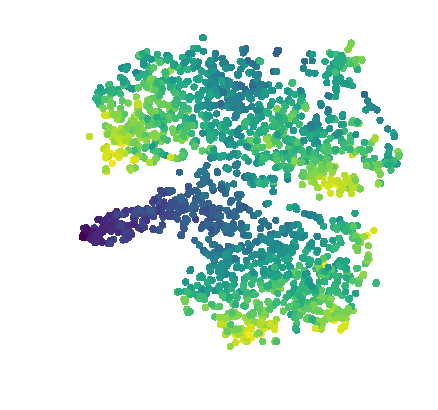
\includegraphics{figures/methods/tsne/thumbs-up}
    \caption{Thumbs up}
  \end{subfigure}
  \begin{subfigure}{0.49\textwidth}
    \centering
    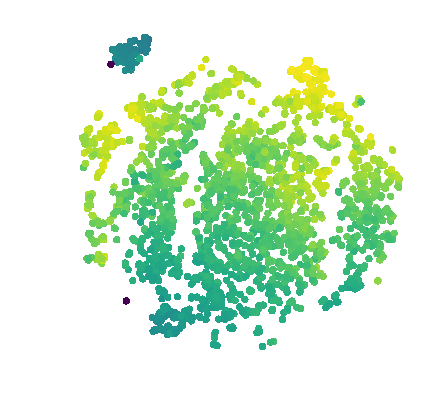
\includegraphics{figures/methods/tsne/swipe-left}
    \caption{Swipe left}
  \end{subfigure}
  \caption{t-SNE plots of learned representations of \SI{2.5}{\milli\second} segments}
  \label{fig:autoencoder}
\end{figure}

% TODO: Maybe explain t-SNE

Figure \ref{fig:autoencoder} shows two t-SNE plots of representations that we
learned with an autoencoder. Each point represents \SI{2.5}{\milli\second} of
events and they are colored by the number of events that went in them where a
brighter color denotes more events. Note that the axes carry no meaning in a
t-SNE plot and all information is in the distance between points. The key
observation is that the points form some high-dimensional structure that
encodes, among others, the event density in a segment.

\section{Framewise Classification}
\label{sec:framewise}

A framewise classification network produces for each sequence element a
multinomial distribution over the classes that encode the network's belief that
an element belongs to a certain class.

% TODO: Architecture with softmax + cross entropy

\begin{figure}[h]
  \centering
  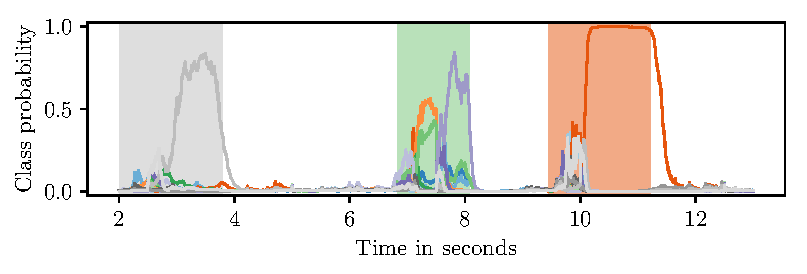
\includegraphics{figures/methods/framewise}
  \caption{Class probabilities attained from framewise classification}
  \label{fig:framewise-p}
\end{figure}

The \texttt{<blank>} class made up about 50\% of the training data and therefore
is the easiest to learn. This is illustrated in Figure \ref{fig:framewise-p}.

\section{Hidden Markov Model Decoding}
\label{sec:hmm}

A framewise classifier tells us which gesture most likely happened at each point
in time but a \texttt{swipe-down} gesture might be classified as
\texttt{rotate-outward} for the first few milliseconds, then \texttt{swipe-up}
for another few and finally as \texttt{swipe-down} for the rest of the gesture.
This sequence of probability distributions now needs to be deciphered into just
a single \texttt{swipe-down} label. The classical approach to this is hidden
Markov model decoding.

% TODO: graphical HMM model with states and emissions

\begin{figure}[h]
  \centering
  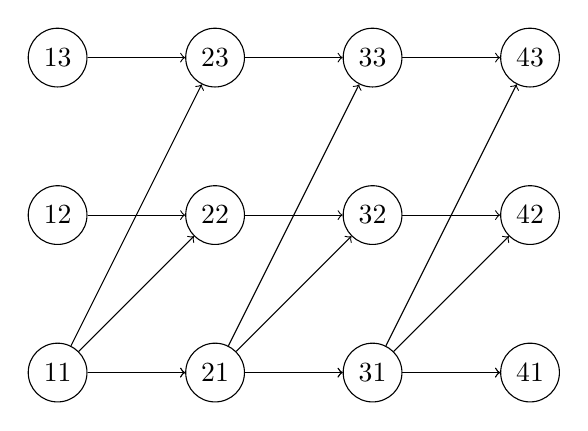
\begin{tikzpicture}[scale=2]
    \foreach \i in {1, 2, 3, 4}
    \foreach \j in {1, 2, 3}
    \node[circle,draw](\i\j) at (\i, \j) {\i \j};

    \foreach \i [evaluate=\i as \inext using int(\i+1)] in {1, 2, 3}
    \foreach \j in {1, 2, 3}
    \draw[->] (\i1) -- (\inext\j);

    \foreach \i [evaluate=\i as \x using int(\i+1)] in {1, 2, 3}
    \foreach \j in {1, 2, 3}
    \draw[->] (\i\j) -- (\x\j);
  \end{tikzpicture}
  \caption{}
  \label{fig:}
\end{figure}

\section{Connectionist Temporal Classification}
\label{sec:ctc}

\begin{figure}[h]
  \centering
  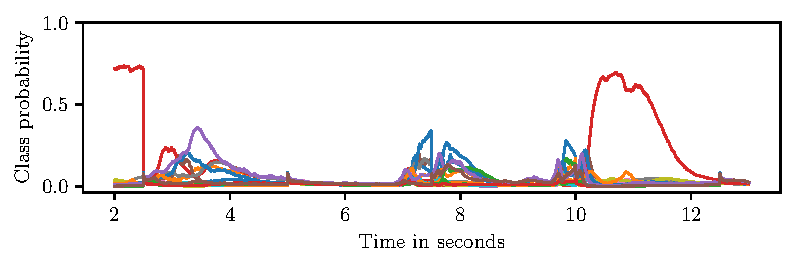
\includegraphics{figures/methods/ctc}
  \caption{Class probabilities attained with CTC}
  \label{fig:ctc-p}
\end{figure}

In the combined approach with neural network and HMM, we train two different
systems in series and the NN.

Training with categorical cross entropy tries to categorize short windows of events correctly.
However, this is not actually what we want and may also be impossible to do.
For example, the gestures extend-index-finger and tap-index-finger start the exact same way, so the first few events are not distinguishable.
With CTC we might be able to get the network to stay quiet until it is sure, which type of gesture it is, instead of forcing it to predict one of them at inappropriate times.

% TODO: Training problems because of long sequences and the need to store all
% intermediate results for BPTT. Sequences without any labels cannot be handled.

% TODO: Chunk size is 250 but RNNs can still learn longer sequences empirically,
% see Graves handwriting paper.
